\documentclass[a4paper,12pt,openright,twoside]{report}
\usepackage[utf8]{inputenc}
\usepackage[italian]{babel}
\usepackage{pdflscape}
\usepackage{afterpage}
\usepackage{esvect}
\usepackage{amsthm}
\usepackage{graphicx}
\usepackage{indentfirst}
\usepackage{stmaryrd}

\theoremstyle{definition}
\newtheorem{es}{Esempio}[section]

\begin{document}

\chapter{Introduzione}
TODO

\chapter{Titolo da decidere}
Lo scopo di questo capitolo è quello di introdurre e descrivere la 
\emph{Sentiment analisys}, chiarendone le caratteristiche, l'ambito di applicazione e 
le peculiarità che ne stanno causando la rapida diffusione. 
Successivamente saranno descritti gli strumenti che sono stati utilizzati per lo svolgimento di questa tesi,
ossia le reti neurali ricorrenti (\emph{RNNLM}), i vector space models (\emph{word2vec}) e 
i classificatori lineari (\emph{Liblinear}).

\section{Sentiment Analisys}
Con il termine \emph{Sentiment analysis}, o \emph{opinion minig}, si intende uno studio 
che analizza le opinioni, i sentimenti, le valutazioni e le
emozioni del linguaggio scritto utilizzato dalle persone.
Spesso il concetto di \emph{sentiment analysis} si estende anche nell'ambito del \emph{data mining} e
\emph{text mining}, ossia quella branca di ricerca riguardante l'estrazione di un sapere o 
di una conoscenza a partire da grandi quantità di dati.

La \emph{Sentiment analysis}, nata nell'ambito dell'informatica, è una delle aree di ricerca più attive 
nel campo dell'analisi del linguaggio naturale e si è diffusa
ampiamente anche in altri rami scientifici come ad esempio: la scienza sociale,
l'economia il marketing. Inoltre questo tipo di ricerca
ha avuto un grande impatto sia a livello commerciale, per aziende e multinazionali, sia sociologico 
coinvolgendo l'intera società che ci circonda.

L'enorme diffusione della \emph{sentiment analysis} coincide con la 
crescita dei cosiddetti \emph{social media}: siti di commercio e recensioni di prodotti,
forum di discussione, blog, micro-blog e di vari \emph{social network}.
Per la prima volta nella storia è possibile disporre di una
enorme quantità di dati digitalizzati. Dati da manipolare, analizzare e studiare in maniera
estremamente approfondita, al fine di estrapolare ed ottenere un'analisi
ampiamente sfaccettata e particolareggiata.

Gli studi di \emph{sentiment analysis} sono applicabili in quasi tutte
le attività del cosiddetto dominio sociale, le opinioni e i pareri 
sono infatti al centro della maggior parte delle attività umane e sono 
altresi la chiave che influenza il nostro comportamento. Sono altresi' la 
chiave che influenza il nostro 
comportamento. Cio' in cui crediamo, la percezione della realtà, le scelte che facciamo
sono condizionate dall’ambiente che ci circonda e dai giudizi 
degli altri riguardo noi stessi.
Per questo motivo, quando abbiamo bisogno
di prendere una decisione, spesso chiediamo il parere e il consenso altrui.
Questo comportamento si verifica non solo 
nei singoli individui, ma lo possiamo  vedere applicato allo stesso modo ad
applicato ad organizzazioni, aziende e grandi multinazionali.
Da tutti questi aspetti è facile dedurre 
come, \emph{la sentiment analysis} possa avere una grande influenza nel mondo che 
ci circonda sia dal punto di vista economico che sociale.

Mentre la linguistica e l'analisi del linguaggio naturale (NLP) hanno una lunga
storia, la \emph{sentiment analysis} è relativamente recente: le prime ricerche
sono state svolte a partire dall'anno 2000. Nonostante questo abito di ricerca sia cosi' giovane 
si presenta come un'area estremamente attiva 
la crescita della ricerca nel campo della \emph{sentiment analysis}, avvenuta in maniera così immediata e su larga scala, 
ha molteplici ragioni. 
Per prima cosa le applicazioni pratiche 
di questo tipo di ricerca sono svariate e possono essere utilizzate in un ampio raggio di 
situazioni e domini differenti. Ciò ha generato un aumento di interesse notevole da parte di
aziende e di grandi multinazionali (non solo in ambito informatico)
con un relativo stanziamento di finanziamenti specifici per questo campo di ricerca.
In secondo luogo il grande interesse dimostrato da parte del mercato ha portato ad una proliferazione di 
applicazioni commerciali e ad una costante ricerca della soluzione di problemi
che fino ad ora non erano ancora stati studiati.

\subsection{Applicazioni della Sentiment Analysis}
Partiamo dunque dal presupposto che le opinioni e i pareri sono la base di tutte le attività sociali,
 essendo la chiave che influenza il nostro comportamento. Nel mondo reale, aziende e multinazionali 
 sono costantemente alla ricerca di giudizi e pareri dati dai consumatori  rispetto ai loro prodotti. 
 Allo stesso modo il consumatore vuole avere informazioni che riguardino gli articoli da acquistare, 
 opinioni inerenti un determinato film o un nuovo album musicale e così via. In passato, quando un’azienda 
 necessitava di un parere del consumatore, effettuava sondaggi d’opinione o gruppi di discussione: 
 ottenere questo tipo di dati è stato per lungo tempo un grande business per aziende di marketing e 
 per compagnie pubblicitarie.
Al giorno d’oggi chiunque voglia comprare un prodotto, potendo trovare centinaia di recensioni o 
discussioni online non è più limitato a dover chiedere informazioni ad amici o famigliari. 
Allo stesso modo le aziende non sono più costrette a condurre sondaggi o analisi di mercato vista 
l’enorme diffusione dei dati disponibili. Tuttavia la ricerca, l’estrazione e l’annotazione di questi 
dati è un compito di una complessità non indifferente, basti pensare alla quantità di informazioni 
scritte nel post di un blog o in un forum, che rendono difficoltosa anche ad un singolo l'elaborazione 
e la sintesi delle informazioni utili: ecco perché diventa cosi importante uno studio finalizzato e 
strutturato in un determinato ambito.


\section{Recurrent Neural Networks}
Gli esseri umani non iniziano a pensare da zero: esiste infatti per la mente umana una capacità di 
associare tra loro informazioni passate e recenti che è stata definita \emph{persistenza della memoria.} 
Il lettore di questa tesi, ad esempio, assocerà il significato di ogni parola basandosi su quelle 
lette in passato.
Le reti neurali tradizionali, al contrario,  ignorano gli eventi passati. Volendo prendere ad esempio 
la classificazione della successione delle scene di un film, non è possibile che una rete neurale 
possa utilizzare gli eventi passati per classificare quelli correnti.

Per cercare di risolvere questo problema sono state create le \emph{recurrent neural networks (RNN)}:
a differenza delle reti neurali tradizionali le \emph{RNN} hanno dei cicli interni che permettono
all'informazione di persistere.

\begin{figure}[ht]
	\centering
	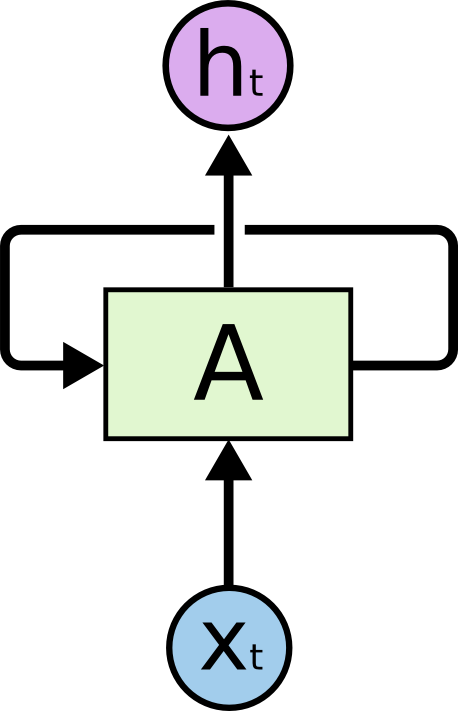
\includegraphics[scale=0.5]{Immagini/rnn1.png}
	\caption{Ciclo interno di una RNN}
	\label{fig:rnn1}
\end{figure}

Nella figura \ref{fig:rnn1}, è rappresentata una rete neurale $A$ che riceve in input un valore $x_t$ e genera in output un valore $h_t$.
Un ciclo permette all'informazione di passare da ogni step della rete al successivo. 
In altro parole possiamo immaginare
una \emph{RNN} come molteplici copie della stessa rete, ognuna delle quali passa un messaggio alla rete successiva.

\begin{figure}[ht]
	\centering
	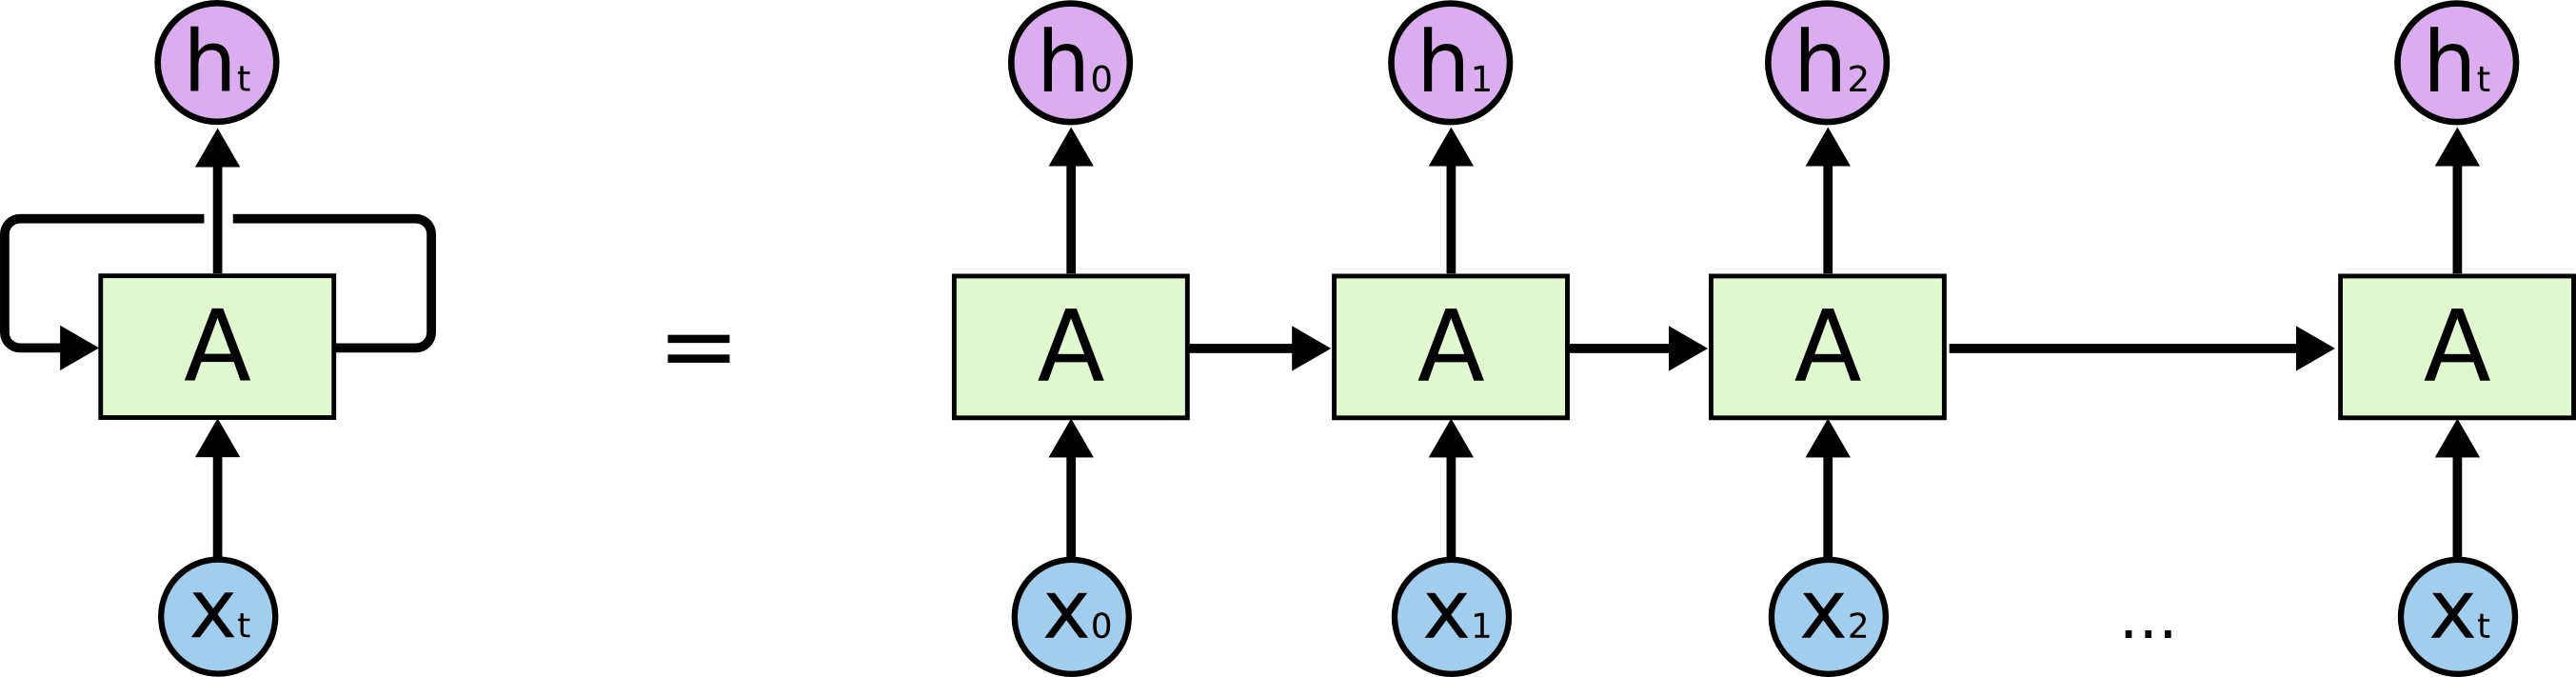
\includegraphics[scale=0.3]{Immagini/rnn2.png}
	\caption{Esempio di RNN \emph{unfolded}, cioè senza cicli}
	\label{fig:rnn2}
\end{figure}

In sostanza una \emph{RNN} riceve come input un vettore $x$ e come output un vettore $y$ ma il cuore della rete
è dato dal fatto che l'output viene influenzato non solo dall'ultimo input acquisito ma anche da tutti gli 
input passati. Se volessimo esprimere questo concetto sotto forma di codice avremo una definizione di \emph{RNN}
che è la seguente:
\begin{verbatim}
rnn = RNN()
y = rnn.step(x)
\end{verbatim}
La \emph{RNN} possiede uno stato interno che viene aggiornato ad ogni esecuzione della procedura \emph{step}.
Per esempio una funzione di \emph{step} potrebbe essere implementata come segue:
\begin{verbatim}
class RNN:
  # ...
  def step(self, x):
    # aggiornamento dello stato interno
    self.h = np.tanh(np.dot(self.W_hh, self.h) 
           + np.dot(self.W_xh, x))
    # calcolo del vettore di output
    y = np.dot(self.W_hy, self.h)
    return y
\end{verbatim}

Si può notare come la \emph{RNN} utilizzi tre parametri: \emph{W\_hh, W\_xh, W\_hy}, inizializzato a zero
è \emph{self.h} e la funzione \emph{np.tanh} fornisce come output un valore che oscilla tra $[-1,1]$.
All'interno di questa funzione notiamo due termini, uno che si basa sullo stato dell'input attuale e uno che 
rappresenta il valore dello stato interno precedente. I due termini vengono sommati prima di essere processati dalla 
funzione stessa.

\subsection{RNNLM}
La rete neurale utilizzata per l'analisi dei dati in questa tesi è il toolkit RNNLM. 
L'architettura utilizzata nel toolkit, mostrata in \ref{fig:rnnlm} viene solitamente chiamata rete di Elman o semplicemente RNN. 
Il \emph{layer} di input usa una rappresentazione $1-a-N$ delle 
parole precedenti $w(t)$ concatenate con il precedente stato dell'hidden layer $s(t - 1)$.
\begin{figure}[ht]
  \centering
      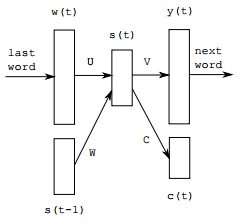
\includegraphics[width=0.5\textwidth]{Immagini/rnnlm_rete.png}
      \caption{Esempio di rete neurale ricorsiva}
\label{fig:rnnlm}
\end{figure}

I neuroni dell'\emph{hidden layer} $s(t)$ usano una funzione sigmoidea, cioè una funzione matematica
che produce una curva sigmoide (una curva avente un andamento ad $S$).

\begin{figure}[ht]
  \centering
      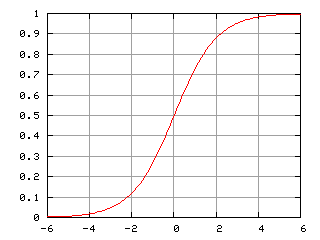
\includegraphics[width=0.5\textwidth]{Immagini/sigmoide.png}
      \caption{Esempio di grafico di una funzione sigmoidea}
\label{fig:sigmoide}
\end{figure}

Questo tipo di funzione viene utilizzata per introdurre una non linearità nel modello e per
assicurarsi che determinati  valori rimangano all'interno di specifici intervalli.
Dopo il training della rete l'output layer $y(t)$, che ha le stesse dimensioni di $w(t)$,
rappresenta la probabilità della distribuzione della parola $n+1$ partendo dalla parola $n$ 
e lo stato dell'\emph{hidden layer} nel precedente istante di tempo.
Un class layer $c(t)$ può essere usato per ridurre la complessità del modello ma con un piccola
diminuzione della precisione.
Il training viene svolto utilizzando un \emph{stochastic gradient descent algorithm}, cioè utilizzando
una funzione di ottimizzazione locale scritta sotto forma di funzioni differenziali. La matrice $W$
che rappresenta il \emph{recurrent weights} (il peso degli stati passati) viene calcolata utilizzando la 
\emph{backpropagation throught time algorithm (BPTT)}.
Specificatamente, su RNNLM, viene utilizzato un truncate BPTT, la rete cioe' processata solo per uno specifico
numero di istanti di tempo.

\subsection{Fase di training}
Nella fase di training i dati in ingresso sono attesi sotto forma di un semplice file ASCII: ogni parola
deve essere separata da spazi e deve essere presente il carattere di
fine linea al termine di ogni frase.
Una volta specificato il corpus di input, il vocabolario viene costruito automaticamente e viene salvato insieme 
al file di modello generato da RNNLM.
Questo significa che, nel caso si voglia limitare il vocabolario, il file di input deve essere modificato in maniera
preventiva, sostituendo
tutte le parole da eliminare con un token speciale (per esempio \textbf{\textless unk \textgreater}).
Oltre al corpus, per completare la fase di training è atteso anche un
file di validazioni dati per regolare il numero di training \emph{epochs} da utilizzare e  il learning rate.
\`E anche possibile fare training di modelli senza utilizzare un file di validazione tramite l'opzione \textbf{-one-iter}.
\subsection{Fase di test}
Una volta effettuato il training il modello può essere utilizzato per valutare dati di test:
l'output di questa valutazione è espresso come \emph{perplexity} (la misura di quanto un modello probabilistico
si avvicina al valore di test) e la 
probabilità $\log_{10}$.
Dato il modello e', possibile effettuare una interpolazione lineare delle probabilità delle parole dato il modello. L'input atteso
da RNNLM è un file contenente una lista di frasi, ognuna anteposta con un identificatore
numerico univoco, su cui effettuare lo scoring.

\section{Word2Vec}
Storicamente i sistemi di \emph{natural language processing} trattano le parole come simboli atomici e discreti:
per esempio la parola ``gatto'' può essere rappresentata da \textbf{Id123} e la parola ``cane'' come \textbf{Id453}.
Questa codifica è arbitraria e non fornisce alcuna informazione al sistema riguardo la relazione
che può esistere tra due differenti simboli.
Questo significa che il nostro sistema non può utilizzare praticamente nulla di quello che ha imparato
riguardo la parola ``gatto'' quando sta processando i dati riguardanti ``cane'' (per esempio il fatto che siano
entrambi animali, che abbiano quattro zampe, etc.).
Inoltre, rappresentare le parole sotto forma di identificatori univoci porta ad avere una base dati sparsa
con la conseguente necessità di dover ottenere un maggior numero di dati per riuscire a creare un modello
statistico rappresentativo; proprio questa base dati sparsa è il principale problema 
ad essere risolto dalla rappresentazione tramite vettori risolve.

\subsection{Vectors space model}
I \emph{Vectors space models (VSM)} sono rappresentazioni \emph{embedding} di parole in uno spazio vettoriale 
continuo, ovvero un'area in cui le parole
semanticamente simili sono mappate in punti vicini: questo metodo si basa sulla \emph{distributional hypotesis}, 
cioè sul fatto che parole che appaiono in 
un determinato contesto condividono lo stesso significato semantico.

La rappresentazione di parole in uno spazio vettoriale aumenta le performance
di un task di analisi del linguaggio naturale. Una delle prime
applicazioni in questo campo risale al 1986 con la ricerca di Rumelharth, Hinton and Williams.
Questa idea è stata successivamente utilizzata in maniera diffusa, trovando ampia 
applicazione in modelli di ricognizione del parlato,
di traduzione automatica, nonché di numerosi altri tasks.

Recentemente, Mikolov et al. hanno introdotto il modello skip-gram 
un metodo efficiente per ottenere
rappresentazioni vettoriali di parole provenienti da un grande numero di dati testuali non strutturati.

\begin{figure}[h]
	\centering
	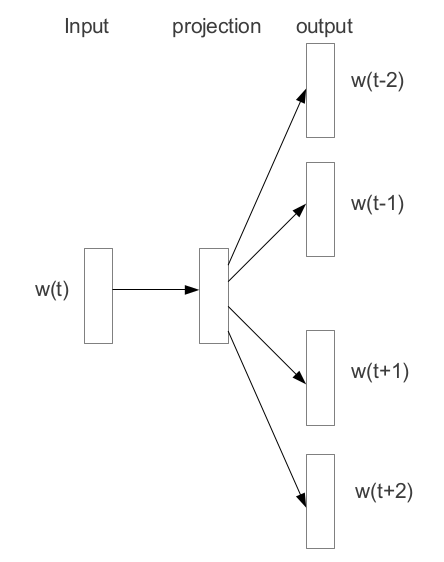
\includegraphics[scale=0.4]{Immagini/skipgram.png}
	\caption{modello Skipgram. L'obbiettivo è ottenere vettori di parole capaci di prevedere
	parole simili}
	\label{fig:skipgram}
\end{figure}

Il training, servendosi di un modello Skip-gram  per la creazione di vettori di parole, 
non utilizza moltiplicazioni tra matrici dense, al contrario della maggioranza delle reti 
neurali: in questo modo diventa estremamente efficiente, in quanto una singola macchina può 
calcolare vettori partendo da un testo contenente più di 100 miliardi di parole in meno di un giorno.   

\subsection{Modello Skip-gram}
Nel modello Skip-gram l'obiettivo di training è quello di creare un vettore di parole che
può essere utilizzato per prevedere vocaboli attorno ad una frase o ad un documento. Più formalmente,
data una sequenza di parole $w_1,w_2,w_3,\dot{},w_T$ definita come training set, 
l'obbiettivo del modello è quello di aumentare la
probabilità logaritmica:
\begin{equation}
	\frac{1}{T} \sum_{t=1}^{T} \sum_{-c\leq j\leq c,j\neq0} \log p(w_t+j|w_t)
	\label{eq:prob log}
\end{equation}
dove $c$ è la dimensione del contesto di training (che può essere una funzione basata sulla parola centrale $w_t$).
Utilizzare un $c$ più grande porta ad avere una precisione maggiore. In questo modo, però, si aumenta anche il 
tempo di calcolo. La formulazione standard del modello Skip-gram definisce $p(w_t+j|w_t)$ usando la funzione
softmax:
\begin{equation}
	p(w_O|w_I) = \frac{\exp(v_{w_O} v_{w_I}}{\sum_{w=1}^{W}\exp(v_w v_{w_I}}
	\label{eq:softmax}
\end{equation}

dove $v_w$ and $v'_w$ sono la rappresentazione vettoriale di ``input'' e ``output'' di $w$, mentre $W$ è il numero
di parole nel vocabolario.
Questa formulazione, però, è difficilmente utilizzabile in sistemi reali
perché il costo per il calcolo di $\nabla\log p(w_O|w_I)$
è proporzionale a $W$, che spesso è molto grande: $(10^5-10^7 termini)$.

\subsection{Hierarchical Softmax}
Una approssimazione del softmax che è computazionalmente più efficiente è il softmax gerarchico. Questo algoritmo
è stato introdotto nell'analisi del linguaggio naturale da Morin e Bengio; il motivo principale
per cui questo algoritmo è più performante rispetto all'algoritmo classico
perchè, per ottenere distribuzione di probabilità, non deve valutare tutti i $W$
 nodi di output della rete neurale, ma solo un numero  $\log_2(W)$ di nodi.

Il softmax gerarchico utilizza una rappresentazione ad albero binario per il \emph{layer} di output 
in cui, come foglie,
troviamo le $W$ parole e, in ogni nodo, la rappresentazione delle probabilità dei nodi figli.
Questo definisce una \emph{random walk} per assegnare la probabilità alle parole.

Più precisamente ogni parola $w$ può essere raggiunta da un determinato percorso partendo dalla radice
dell'albero. Definiamo $n(w,j)$ come il $j$-esimo nodo nel percorso che parte dalla radice fino a $w$ e $L(w)$ come
la lunghezza di questo percorso in modo che $n(w,1) = radice$ e $n(w,L(w)) = w$.
In aggiunta, per ogni nodo interno $n$, definiamo $ch(n)$ come un arbitrario nodo figlio di $n$ e $[x]$ ha il valore $1$ se $x$ è vero e $-1$ altrimenti.
Quindi il softmax gerarchico definisce $p(w_O|w_I)$ come segue:
\begin{equation}
	p(w|w_I) = \prod_{j=1}^{L(w)-1}\sigma([n(w,j+1)=ch(n(w,j))]\dot v_{n(w,j)} )
	\label{eq:hierarchicalSoftmax}
\end{equation}

dove $\sigma(x) = 1/(1+exp(-x))$. Può essere dimostrato che $\sum_{w=1}^W p(w|w_I) = 1$. Questo implica
che il costo per calcolare $\log p(w_O|w_I)$ e $log p(w_O|w_I)$ è proporzionale a $L(w_O)$ che in media
è più piccolo di $\log W$.
Inoltre, al contrario della formulazione stardand del softmax dove troviamo due rappresentazioni differenti 
$v_w e v_w$ per ogni parola $w$, il softmax gerarchico possiede una sola rappresentazione $v_n$ per ogni nodo $n$
dell'albero binario.

Il tipo di albero utilizzato ha una influenza notevole sulle prestazioni dell'algoritmo, nello specifico
in word2vec è stato utilizzato un albero binario di Huffmann. In questo modo 
abbiamo codici di dimensioni più piccole per le parole usate con maggior frequenza,
determinando un training più rapido.
Inoltre è stato osservato che raggruppare le parole utilizzando la loro frequenza funziona molto
bene come tecnica per aumentare la velocità di calcolo.

\section{Classificatori lineari}
La risoluzione di problemi di classificazione su una mole molto grande di dati è uno dei problemi principali
incontrati in applicazioni quali la classificazione di testi.

Un classificatore lineare, nel campo dell'apprendimento automatico, è diventato una delle tecnologie più
promettenti e più utilizzate: l'obiettivo della 
classificazione lineare è quella di usare le caratteristiche degli oggetti (\emph{Features}) per identificare
a quale classe (o gruppo) appartengono. 
Una classificazione lineare raggiunge questo scopo effettuando una decisione sulla classificazione basata sul valore di una combinazione lineare di caratteristiche. 
Le caratteristiche di un oggetto sono anche conosciute come \emph{features} e nel calcolatore sono rappresentati solitamente come un vettore chiamato vettore delle caratteristiche.

Questi classificatori funzionano molto bene per problemi pratici quali la classificazione di 
documenti e più in generale per problemi che utilizzano un numero molto elevato di \emph{features}

Se definiamo un vettore di \emph{features} con l'identificatore $x^\rightarrow$ allora il punteggio di output
è definito come segue:
\begin{equation}
	y=f(w^\rightarrow \cdot x^\rightarrow = f (\sum_j w_jx_j)
	\label{output score}
\end{equation}

dove $w^\rightarrow$ è un vettore reale pesato (\emph{weight vector}) e $f$ è una 
funzione che converte il prodotto scalare di due vettori nell'input desiderato.
Il \emph{weight vector} viene generato partendo da un inseme di esempi utilizzati come training. Solitamente
la funzione $f$ è una semplice funzione
che effettua il mapping di tutti i valori sopra una certa soglia nella prima classe e gli altri valori nella
seconda classe. Una versione più complessa di $f$ potrebbe fornire una probabilità con cui un particolare
oggetto appartiene ad una certa classe.

L'utilizzo dei classificatori lineari avviene spesso in situazioni in cui la velocità di classificazione
è rilevante, specialmente quando $x^\rightarrow$ è sparso.
\begin{figure}[ht]
	\centering
	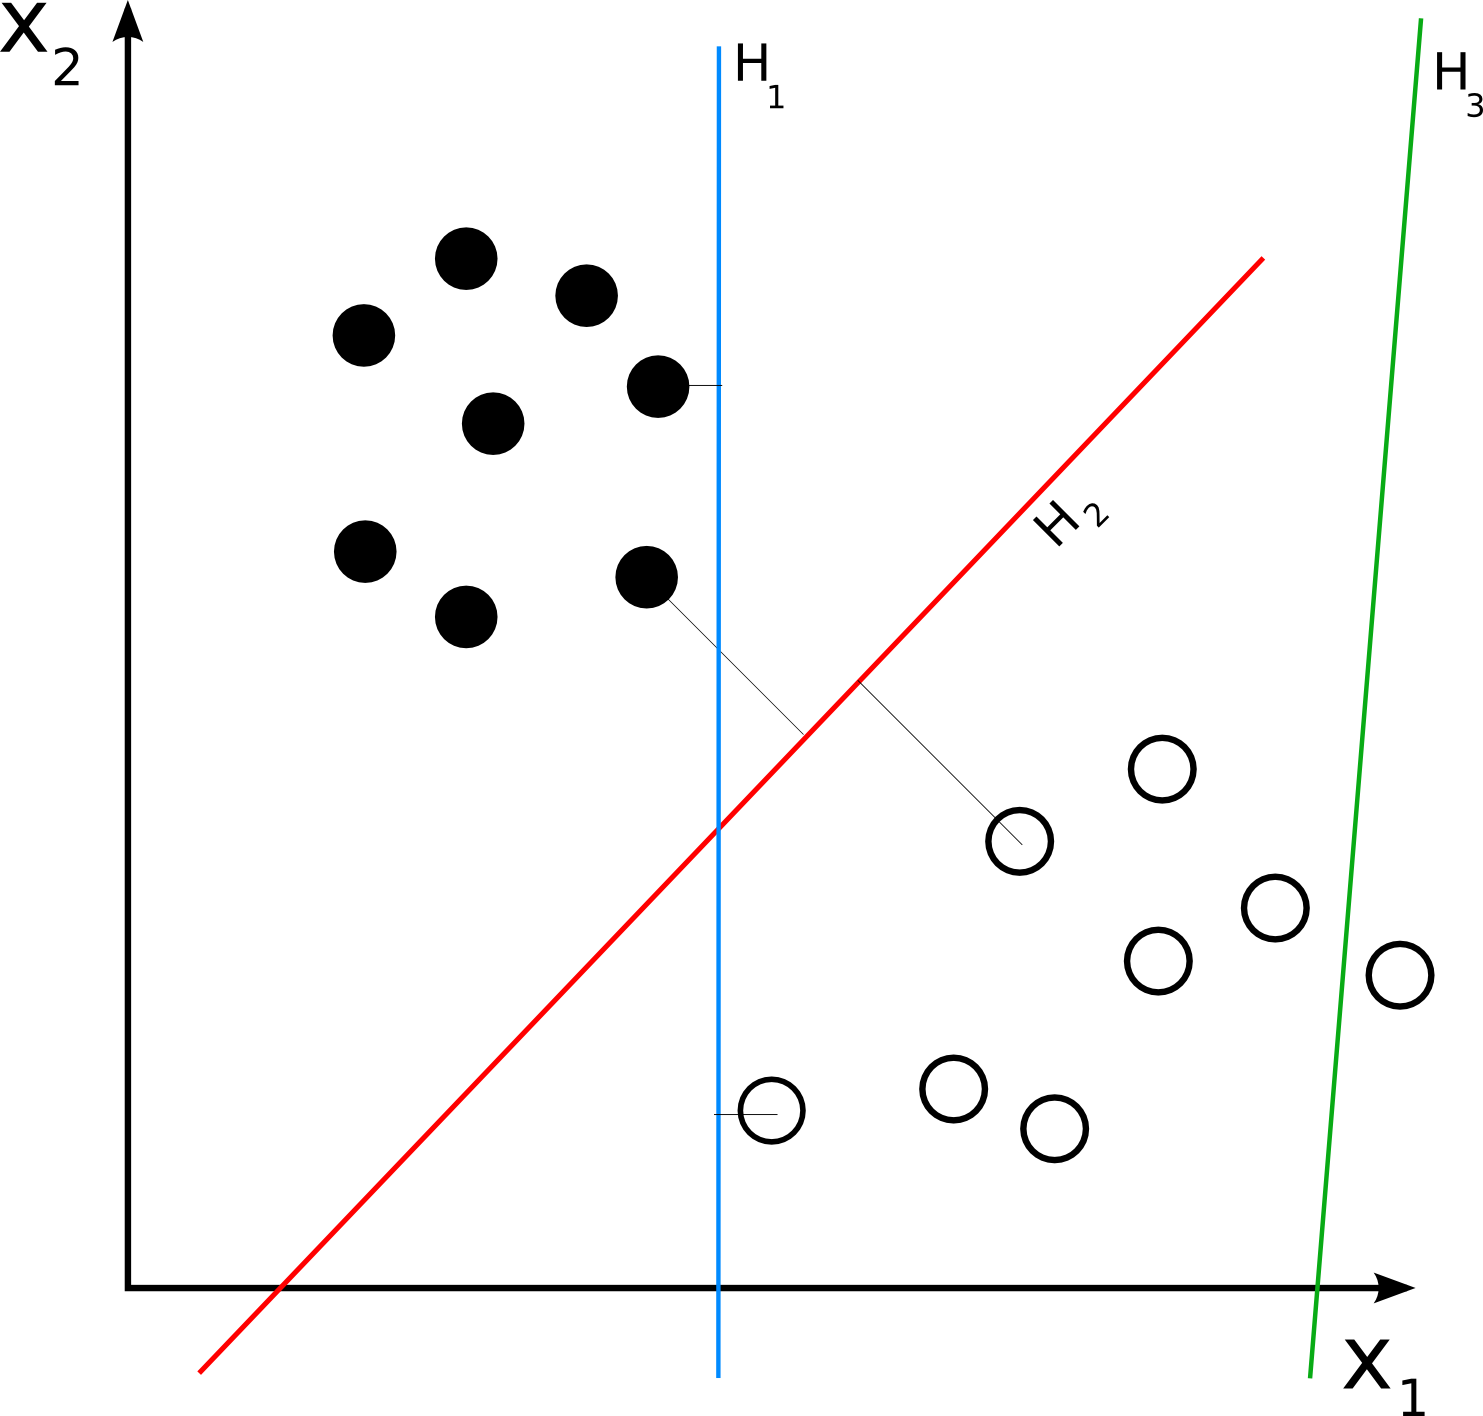
\includegraphics[scale=0.2]{Immagini/liblinear_esempio.png}
	\caption{Nella figura vediamo come il classificatore $H_1$ e $H_2$ classifichino
	correttamente i punti pieni e i punti vuoti. Potremmo dire, inoltre, che $h_2$
	è un classificatore migliore perché la distanza media tra i vari elementi è costante}
	\label{fig:liblinearEx}
\end{figure}

\subsection{Liblinear}
Liblinear è una libreria opensource che implementa algoritmi di classificazione lineare. Il motivo
per cui è stata scelta come strumento per questa
tesi è principalmente dovuto alla sua estesa documentazione, alla semplicità
d'uso, al suo già ampio utilizzo in ricerche simili e infine per la sua velocità nel calco dei risultati. 
In particolare l'ultimo punto si è rivelato fondamentale
per ottenere risultati in tempo ragionevole: in un confronto con un risolutore \emph{SVM} (come \emph{LIBSVM})
i tempi di calcolo vengono ridotti di tre ordini di grandezza (da svariate ore a pochi secondi).

Liblinear supporta due popolari classificatori binari \emph{LR, L2-regularized logistic regression} e 
\emph{SVM L2-loss linear support vector machine}, dato un inseme di coppie
indicizzate $(x_i,y_i),i=1,\dot{},l,x_i\in R^n, y_i \in \{-1,+1\}$ entrambi i metodi risolvono lo stesso
problema di ottimizzazione senza vincoli ma con differenti \emph{loss functions} $\Xi(w;x_i,y_i)$:
\begin{equation}
	min_w \frac{1}{2}w^Tw+C\sum_i=1^l\Xi(w;x_i;y_i)
	\label{eqn:liblinear1}
\end{equation}

dove $C > 0$ è il parametro di penalità. Per \emph{SVM} le due \emph{loss functions} sono $max(1-y_iw^Tx_i,0)$ e
$max(1-y_iw^Tx_i,0)$. Per \emph{LR} invece abbiamo $\log(1+e^{-y_iw^Tx_i}$

Per quanto riguarda l'utilizzo il toolkit di Liblinear fornisce due diversi eseguibili \emph{train} e 
\emph{predict}.
L'eseguibile \emph{train} viene utilizzato per la creazione del modello e acquisisce, come input, un file
ASCII suddiviso per righe. In particolare, per questa tesi, e' stato usato come algoritmo 
per il training del modello ottenuto tramite \emph{logistic regression}.
Utilizzando la \emph{regressione lineare} e' possibile utilizzare l'eseguibile \emph{predict} in modo 
che fornisca in output le stima delle probabilita' per ogni riga.

\chapter{Raccolta dati}
La raccolta dati è stata svolta svolta partendo dal primo Gennaio 2015, i dati raccolti provengono da dodici canali twitch scelti in modo che rappresentassero un parte omogenea di informazioni.
In particolare sono stati scelti i due canali con maggiore audience dei quattro giochi con maggiore numero di spettatori della piattaforma Twitch.tv.
I canali sono tutti in lingua inglese e i dati sono stati raccolti modificando logging per IRC  in modo che potesse raccogliere dati attraverso il login e l'utilizzo dell API di twitch.
Oltre al messaggio di testo sono stati registrati anche l'autore (utente) del messaggio di testo, il timestamp e il canale nel quale il messaggio è stato inserito.

\section{Normalizzazione del corpus}
Dato il grande numero di dati e il fatto che chiunque può partecipare alla chat di Twitch si è reso necessario l'eliminazione degli eventuali messaggi di spam. Il primo step è stato quello di sostituire tutte gli URL presenti con il token \textbf{URL}. 
Il secondo step è stato quello di trasformare tutte le emoticons unicode presenti utilizzando il documento TODO LINK sostituendole con i rispettivi tag ASCII. Un'ulteriore step è stato preso in modo da eliminare caratteri unicode non necessari per esempio lettere straniere proveniennti da altri paesi non anglofoni (esempio \o, \oe, etc.).
Il principale metodo di tokenizzazione è stato fatto utilizzando \textbf{Twoketnizer} (TODO inserire link) un tokenizer sviluppato per tokenizzare testi provenienti da twitter. In particolare è stata utilizzata la sua implementazione in python con alcune modifiche in modo da trattare le emoticons presenti nel corpus di Twitch.

\section{Analisi Emoticons}
Sono state scelte per un'analisi più approfondita le seguenti emoticons:
\begin{table}[h]
\begin{center}
\begin{tabular}{|c|c|c|}
\hline
Nome Emoticon & Significato & Polarity \\
\hline
\hline
4Head & sarcasmo & positiva \\
\hline
anele & sarcasmo, in genere riferito alla cultura USA & neutra \\
\hline
babyrage & insofferenza & negativo \\
\hline
biblethump & disappunto & negativo \\
\hline
brokeback & sarcasmo & positiva \\
\hline
dansgame & critica & negativo \\
\hline
datsheffy & battute sulla polizia (singolo canale) & non considerato \\
\hline
elegiggle & sarcasmo & positiva \\
\hline
pogchamp & spam & non considerato \\
\hline
residentsleeper & noia & negative \\
\hline
smorc & tattiche relative ad un particolare gioco & neutra \\
\hline
swiftrage & rabbia & negativo \\
\hline
trihard & impegno &  neutro \\
\hline
wutface & spam & non considerato \\
\hline
failfish & disappunto & negative \\
\hline
frankerz & spam & non considerato \\
\hline
heyguys & annunci/saluti & positiva \\
\hline
kappa & sarcasmo & positiva \\
\hline
kappapride & sarcasmo & positiva \\
\hline
kreygasm & sarcasmo & positiva \\
\hline
mrdestructoid & battute / viewbotting & neutre \\
\hline
opieop & commenti sul cibo & neutra \\
\hline
osbury & offese & negativo \\
\hline
osrob & spam & non considerato \\
\hline
pjsalt & disappunto & negative \\
\hline
\end{tabular}
\end{center}
\caption{Analisi delle emoticons}
\label{tab:emoticons1}
\end{table}

Si può notare che è possibile divedere le emoticons in quattro classi separate, 
\begin{itemize}
\item Positiva: rappresenta frasi ironiche, sarcastiche e che esprimono un apprezzamento sul contenuto del canale.
\item Negativa: rappresenta un giudizio negativo sul contenuto del canale o su argomenti trattati in chat.
\item Neutra: sono emoticons che non hanno una polarity definita, in questa classe troviamo emoticons, per esempio opieop, utilizzate in frasi che parlano di cibo "I'm getting an hamburger now opieop" frasi che quindi sono scollegate dall'argomento dello streaming o della chat. In questa classe troviamo anche emoticons come mrdestructdroid che viene utilizzato principalmente per indicare il cosidetto "viewbotting" cioè l'utilizzo di software che crea connessioni fittizie allo streaming in modo da incrementare il numero di visualizzazioni in modo da far salire il ranking dello stream stesso. L'analisi di questo comportamento, anche se molto interessante, esula dagli argomenti trattati in questa tesi pertanto viene ignorato.
\item Non considerata: in questa classe troviamo le emoticons che non esprimono alcun giudizio, sono utilizzate spesso solo per creare "confusione" nella chat. TODO spiegare meglio
\end{itemize}

\begin{table}[h]
\begin{center}
\begin{tabular}{|c|c|c|}
\hline
Positive & Negative & Non considerate/Neutre \\
\hline
4Head & babyrage & datsheffy \\
\hline
anele &  biblethump &  pogchamp \\
\hline
brokeback &  dansgame & smorc \\
\hline
elegiggle & residentsleeper &  swiftrage \\
\hline
heyguys & failfish & trihard \\
\hline
kappa & pjsalt & wutface \\
\hline
kappapride & osbury & frankerz \\
\hline
kreygasm &  & keepo \\
\hline
 & & mrdestructoid \\
\hline
& & opieop \\
\hline
& & osrob \\
\hline
\end{tabular}
\end{center}
\caption{Lista di emoticons raggruppata per polarity}
\label{tab:emoticons2}
\end{table}

\chapter{Rnnlm}
\label{ch:rnnlm}
Seguento gli esempi pubblicati da Mikolov dove utilizza dati provenienti da IMDB e dimostra che un  modello generativo creato utilizzando recurrent neural network  può essere utilizzato per fare classificazione. Seguento lo stesso esempio sono creati modelli per ogni emoticons prendendo 15000 righe in modo casuale poi testati su un corpus di test composto da 25000 righe (diverse da quelle utilizzate come train).
Sono state prese 4 emoticons normalmente usate per esprimere un parere positivo e 6 per esmprimere un parere negativo e confrontate fra loro. Nelle tabelle sono rappresentate le percentuali di accurancy ottenuto sul file di test
\begin{table}[h]
\begin{center}
\begin{tabular}{|c|c|c|c|c|c|c|}
\hline
pos/neg & Babyrage & Biblethump & Dansgame & Failfish & notlikethis & wutface \\
\hline
\hline
4Head & 82.01 &  79.322 & 78 & 77 & 82.5 & 80.202 \\
\hline
Elegiggle & 84.372 & 83.696 & 80.794 & 77.454 & 84.7 & 84.288 \\
\hline
Kappa & 83.394 & 79.548 & 79.906 & 78.12 & 84.162 & 83.37 \\
\hline
Kreygasm & 84.944 & 81.964 & 80.388 & 82.228 & 84.608 & 81.114 \\
\hline
\end{tabular}
\end{center}
\caption{Confronto emoticons positive e negative}
\label{tab:rnnlmTest1}
\end{table}

Nello steso modo sono state confrontate le emoticon positive fra di loro
\begin{table}[h]
\begin{center}
\begin{tabular}{|c|c|c|c|c|}
\hline
pos/pos & 4Head & Elegiggle & Kappa & Kreygasm \\
\hline
\hline
4Head & 49.87 &  72.42 & 73.68 & 77.37 \\
\hline
Elegiggle & 72.126 & 50.37 & 78.58 & 81.98 \\
\hline
Kappa & 73.97 & 78.76 & 49.70 & 78.178 \\
\hline
Kreygasm & 77.41 & 82.8 & 79.178 & 49.62 \\
\hline
\end{tabular}
\end{center}
\caption{Confronto emoticons positive}
\label{tab:rnnlmTest2 }
\end{table}

Successivamente sono stati svolti i confronti tra tutte le emoticons positive e tutte quelle negative:
\afterpage{
\clearpage
\thispagestyle{empty}
\begin{landscape}
\centering
\begin{table}[h]
\begin{tabular}{|c|c|c|c|c|c|c|c|c|c|c|c|c|c|c|c|c|c|c|c|c|c|c|c|c|c|c|c|}
 & 4head & anele & babyrage & biblethump & brokeback & dansgame & datsheffy & elegiggle & failfish & frankerz & heyguys & kappapride & kappa & keepo & kreygasm & mrdestructoid & opieop & osbury & osrob & pjsalt & pogchamp & residentsleeper & smorc & swiftrage & trihard & wutface \\
4head &  49.638\% &  85.668\% &  82.05\% &  79.074\% &  76.462\% &  77.964\% &  90.016\% &  71.952\% &  77.076\% &  85.644\% &  85.906\% &  76.828\% &  74.556\% &  73.956\% &  77.214\% &  87.244\% &  79.09\% &  97.264\% &  94.782\% &  81.212\% &  73.688\% &  82.892\% &  &  &  & \\
anele &  &  49.962\% &  90.482\% &  88.012\% &  87.132\% &  88.236\% &  92.522\% &  88.9\% &  89.868\% &  87.402\% &  91.008\% &  85.584\% &  85.946\% &  85.866\% &  86.542\% &  90.804\% &  85.872\% &  97.146\% &  97.204\% &  89.542\% &  87.364\% &  91.866\% &  88.7\% &  90.362\% &  85.904\% &  88.028\%\\
babyrage &  &  &  50.094\% &  82.066\% &  84.308\% &  84.884\% &  93.334\% &  84.246\% &  84.112\% &  88.434\% &  90.384\% &  84.706\% &  83.196\% &  83.19\% &  84.616\% &  90.81\% &  85.408\% &  97.682\% &  96.252\% &  87.872\% &  83.644\% &  88.4\% &  87.298\% &  85.03\% &  89.026\% &  86.298\%\\
biblethump &  &  &  &  50.022\% &  83.162\% &  81.068\% &  91.722\% &  83.44\% &  82.318\% &  85.338\% &  88.02\% &  80.874\% &  79.278\% &  79.388\% &  81.566\% &  88.616\% &  82.164\% &  97.3\% &  95.134\% &  86.636\% &  80.894\% &  86.444\% &  86.02\% &  83.218\% &  86.318\% &  80.704\%\\
brokeback &  &  &  &  &  50.212\% &  80.112\% &  91.712\% &  79.862\% &  77.534\% &  87.13\% &  87.156\% &  80.892\% &  79.338\% &  78.786\% &  78.338\% &  89.308\% &  81.09\% &  96.934\% &  96.326\% &  84.73\% &  79.886\% &  84.766\% &  83.618\% &  86.012\% &  84.808\% &  81.72\%\\
dansgame &  &  &  &  &  &  50.188\% &  91.97\% &  81.268\% &  76.622\% &  87.676\% &  88.26\% &  81.818\% &  80.72\% &  80.136\% &  79.93\% &  89.924\% &  82.37\% &  97.694\% &  94.892\% &  86.99\% &  78.464\% &  85.474\% &  85.972\% &  82.058\% &  86.12\% &  76.998\%\\
datsheffy &  &  &  &  &  &  &  49.976\% &  90.514\% &  92.098\% &  92.186\% &  93.822\% &  91.234\% &  90.942\% &  90.406\% &  91.39\% &  93.002\% &  89.964\% &  98.184\% &  97.336\% &  93.192\% &  90.792\% &  93.486\% &  92.362\% &  92.488\% &  91.832\% &  92.448\% \\
elegiggle &  &  &  &  &  &  &  &  49.942\% &  78.47\% &  89.74\% &  89.276\% &  82.63\% &  79.42\% &  79.698\% &  82.324\% &  89.884\% &  82.878\% &  97.276\% &  94.734\% &  85.352\% &  79.718\% &  85.376\% &  86.694\% &  85.15\% &  87.324\% &  84.292\%\\
failfish &  &  &  &  &  &  &  &  &  49.9\% &  89.344\% &  89.636\% &  83.634\% &  78.926\% &  78.448\% &  81.096\% &  90.666\% &  83.182\% &  97.756\% &  95.738\% &  86.544\% &  80.558\% &  84.358\% &  84.07\% &  85.022\% &  87.616\% &  81.916\%\\
frankerz &  &  &  &  &  &  &  &  &  &  49.89\% &  89.774\% &  83.898\% &  85.302\% &  82.472\% &  87.604\% &  89.27\% &  84.768\% &  97.106\% &  97.068\% &  86.454\% &  87.176\% &  90.716\% &  88.694\% &  90.114\% &  86.466\% &  88.002\%\\
heyguys &  &  &  &  &  &  &  &  &  &  &  49.85\% &  86.042\% &  87.862\% &  86.734\% &  85.712\% &  92.036\% &  87.23\% &  97.426\% &  97.166\% &  90.164\% &  86.326\% &  91.948\% &  91.41\% &  91.314\% &  89.478\% &  88.52\%\\
kappapride &  &  &  &  &  &  &  &  &  &  &  &  50.264\% &  &  75.91\% &  79.28\% &  88.798\% &  80.438\% &  97.046\% &  95.992\% &  84.532\% &  79.836\% &  87.022\% &  85.314\% &  85.18\% &  84.066\% &  82.592\%\\
kappa &  &  &  &  &  &  &  &  &  &  &  &  76.268\% &  49.902\% &  71.292\% &  78.71\% &  87.22\% &  78.298\% &  97.572\% &  95.2\% &  84.958\% &  77.112\% &  84.758\% &  82.486\% &  84.074\% &  84.852\% &  82.796\%\\
keepo &  &  &  &  &  &  &  &  &  &  &  &  &  &  50.368\% &  78.54\% &  87.052\% &  77.286\% &  97.492\% &  96.352\% &  83.93\% &  78.416\% &  85.408\% &  82.802\% &  84.166\% &  83.648\% &  82.418\%\\
kreygasm &  &  &  &  &  &  &  &  &  &  &  &  &  &  &  50.004\% &  87.99\% &  81.662\% &  97.566\% &  95.404\% &  85.918\% &  71.374\% &  85.754\% &  84.664\% &  83.842\% &  83.504\% &  81.59\%\\
mrdestructoid &  &  &  &  &  &  &  &  &  &  &  &  &  &  &  &  49.868\% &  89.116\% &  97.898\% &  97.268\% &  91.098\% &  89.688\% &  91.228\% &  90.71\% &  90.454\% &  89.44\% &  90.524\%\\
opieop &  &  &  &  &  &  &  &  &  &  &  &  &  &  &  &  &  49.73\% &  97.68\% &  95.226\% &  86.306\% &  80.384\% &  87.346\% &  85.158\% &  87.116\% &  83.586\% &  84.342\%\\
osbury &  &  &  &  &  &  &  &  &  &  &  &  &  &  &  &  &  &  49.96\% &  98.856\% &  97.538\% &  97.518\% &  98.064\% &  97.954\% &  97.672\% &  97.298\% &  97.424\%\\
osrob &  &  &  &  &  &  &  &  &  &  &  &  &  &  &  &  &  &  &  49.988\% &  96.822\% &  96.118\% &  97.134\% &  95.87\% &  96.11\% &  96.548\% &  96.582\%\\
pjsalt &  &  &  &  &  &  &  &  &  &  &  &  &  &  &  &  &  &  &  &  50.068\% &  85.194\% &  89.502\% &  88.208\% &  89.998\% &  87.598\% &  87.048\%\\
pogchamp &  &  &  &  &  &  &  &  &  &  &  &  &  &  &  &  &  &  &  &  &  50.348\% &  85.058\% &  84.184\% &  81.532\% &  85.13\% &  80.16\%\\
residentsleeper &  &  &  &  &  &  &  &  &  &  &  &  &  &  &  &  &  &  &  &  &  &  50.17\% &  88.79\% &  88.07\% &  89.22\% &  87.948\%\\
smorc &  &  &  &  &  &  &  &  &  &  &  &  &  &  &  &  &  &  &  &  &  &  &  49.91\% &  86.068\% &  87.62\% &  86.966\%\\
swiftrage &  &  &  &  &  &  &  &  &  &  &  &  &  &  &  &  &  &  &  &  &  &  &  &  49.776\% &  89.082\% &  85.906\%\\
trihard &  &  &  &  &  &  &  &  &  &  &  &  &  &  &  &  &  &  &  &  &  &  &  &  &  50.014\% &  84.77\%\\
wutface &  &  &  &  &  &  &  &  &  &  &  &  &  &  &  &  &  &  &  &  &  &  &  &  &  &  49.804\%\\
\end{tabular}
\caption{Confronto emoticon globale}
\label{tab:rnnlmTest3 }
\end{table}
\end{landscape}
\clearpage
}

In questo modo è facile notare che non solo rnnlm riesce a distinguere con alta probabilita  tra frasi provenienti da emoticons positive e quelle da emoticons negative. Ma riesce anche a distinguere con elevata precisione anche le differenze tra due diverse emoticons positive.
\chapter{Liblinear}
\label{ch:liblinear}
Per generare i risultati attraverso liblinear è stato utilizzato word2vec con la patch di Mikolov per i sentence vectors. Similmente da come è stato effettuato con rnnlm sono stati creati file di training e test partendo dalle frasi derivate da due differenti emoticons, una positiva e un'altra negative contenenti 12500 righe ciascuno. Successivamente sono stati creati i file di test di lunghezza 25000 righe. Nonostante nei test sia stato utilizzato un sottoinsieme dei dati i vettori sono stati creati utilizzando l'intero corpus.
Sono state effettuate alcune prove cambiando la lunghezza dei vettori (da 100 a 300 elementi) e anche utilizzando sia l'algoritmo c-bow che continous skipgram. Non sono state osservate particolari differenze nei risultati, per questo motivo si è scelto di utilizzare vettori da 100 elementi e l'algoritmo skipgram.
Come effettuato nel Capitolo 2 sono state effettuati i confronti tra coppie di emoticons positive e negative:

\begin{table}[h]
\begin{center}
\begin{tabular}{|c|c|c|c|c|c|c|}
\hline
pos/neg & Babyrage & Biblethump & Dansgame & Failfish & notlikethis & wutface \\
\hline
\hline
4Head & 67.01 &  69.322 & 78 & 67 & 65.5 & 70.202 \\
\hline
Elegiggle & 69.37 & 71.696 & 70.74 & 67.54 & 69.7 & 68.28 \\
\hline
Kappa & 70.94 & 69.548 & 69.906 & 68.12 & 68.162 & 71.37 \\
\hline
Kreygasm & 69.44 & 71.96 & 70.33 & 72.43 & 67.76 & 71.32 \\
\hline
\end{tabular}
\end{center}
\caption{Confronto emoticons positive e negative}
\label{tab:liblinearTest1}
\end{table}

Sono stati effettuati anche alcuni test utilizzando tutti i vari algoritmi disponibili da liblinear; questo test è stato svolto utilizzando tutti i parametri di default e testato con tutti gli algoritmi la seconda colonna rappresenta i risulati ottenuti con -c 2
\begin{table}[h]
\begin{center}
\begin{tabular}{|l|c|r|}
\hline
Algoritmo & c  default & -c 2 \\
\hline
\hline
0 & 66.9 & 66.88\\
\hline
1 & 66.93 & 66.95\\
\hline
2 & 66.93 & 67.14\\
\hline
3 & 67.16 & 67.24\\
\hline
4 & 67.15 & 66.93\\
\hline
5 & 66.94 & 66.90\\
\hline
6 & 66.9 & 66.84\\
\hline
7 & 66.90 & 66.89\\
\hline
11 & 66.93 & 66.93\\
\hline
12 & 66.47 & 66.63\\
\hline
13 & 65.188 & 67.02\\
\hline
\end{tabular}
\end{center}
\caption{test liblinear}
\label{tab:liblineraTest1}
\end{table}

Il parametro C è stato ricercato utililzzando la funzionalità di liblinear -C: ./train -s 0 -C train.txt . Il risultato ottenuto è stato un c pari a 2. Un ulteriore test utilizzando l'algoritmo 2 e modificando i c da 1 a 4 non ha portato alcuna differenza nei valori di precisione.

TODO inserire i grafici creati con t-sne per la vicinanza delle emoticons

\chapter{Risultati}
I test conclusivi per la classificazione di polarità sono stati effettiati eseguendo sia \textbf{rnnlm} e poi successivamente \textbf{word2vec e liblinear} sullo stesso set di dati. Da come è stato possibile leggere nei capitoli precedenti sono stati eseguiti due test: il primo utilizzando i dati della tabella  \ref{tab:rnnlmTest1}, mentre il secondo è stato svolto utililzando tutte le emoticons positive e negative descritte nella tabella \ref{tab:emoticons1}. 
I test sono stati sempre svolti con un corpus di training di 12500 righe per file (file positivo e negativo) scelte casualmente tra tutto il corpus e un test di 25000 per file. I sentence vectors sono stati generati utililzando l'intero corpus di emoticons positive, negative e neutre non limitato al numero di righe prese in considerazione per i file di training e test.
I risultati ottenuti sono i seguenti:
\begin{table}[h]
\begin{center}
\begin{tabular}{|c|c|c|c|}
\hline
& rnnlm & c liblinear & totale \\
\hline
no ripetizioni 1 & 72.53 & 66.50 & 75.85  \\
\hline
no ripetizioni 2 & 73.34 & 67.50 & 74.85  \\
\hline
no ripetizioni 3 & 72.13 & 66.78 & 75.01  \\
\hline
standard 1 & 74.52 & 67.01 & 78.89 \\
\hline
standard 2 & 75.33 & 69.23 & 81.01 \\
\hline
standard 3 & 74.92 & 68.33 & 79.90 \\
\hline
\end{tabular}
\end{center}
\caption{test liblinear}
\label{tab:test1}
\end{table}

In questo caso sono stati ripetuti 3 volte i test, utilizzando un set di dati di training e test diverso per ogni test. In particolare è stato effettuato un set test rimuovendo le ripetizioni nelle stasse frase. Questo meccanismo, oltre ad alterare il corpus originale, porta a valori di precisione leggermente inferiori e quindi è stato scartato dai successivi test.
\begin{es}
Eliminazione di ripetizione: In una frase contenente le seguenti parole:  ``Good Game Kappa Good Game Kappa Good Game Kappa`` è stata ridotta eliminando le parole ripetute ad una frase del tipo ``Good Game Kappa``.
\end{es}

\section{Analisi di più emoticons}
E' stato suddiviso il corpus in due parti: una parte contenente tutte le frasi positive: cioè quelle contenenti una delle emoticons citate nella tabella \ref{tab:rnnlmTest1} e quello negativo costriuto in egual modo ma utilizzando le frasi marcate con emoticons negative. Questi due set di dati sono statati randomizzati in modo che le frasi proveninenti dalle differenti emoticons venissero considerate con uguale probabilità. Sono state prese 25000 righe da entrambi i file ed effetuando lo stesso procedimento utilizzato nei capitoli \ref{ch:rnnlm} e \ref{ch:liblinear} è stato fatto il training sia con rnnlm che con liblinear, dopo aver processato i vettori (costruiti con l'intero corpus positivo, negativo e neutro).
I test sono stati effettuati utilizzando altre 25000 righe provenienti da entrambi i file positivi e negativi (tutte frasi differenti da quelle utilizzate per il training). Il risultato ottenuto è riportato nella tabella \ref{tab:test2}.
\begin{table}[h]
\begin{center}
\begin{tabular}{|c|c|c|c|}
\hline
& rnnlm & c liblinear & totale \\
\hline
\hline
Test 1 & 54.20 & 52.32 & 53.30 \\
\hline
Test 2 & 53.32 &  51.50 &  53.85  \\
\hline
Test 3 & 53.20 & 52.01 &  51.89 \\
\hline
\end{tabular}
\end{center}
\caption{test liblinear}
\label{tab:test2}
\end{table}

I risultati cosi bassi sono dovuti al fatto che, anche se concettualmente le emoticons positive esprimono una polarità positiva in realtà la costruzione delle frasi associate sono molto diverse. 
In altre parole il sistema si ``confonde`` tra le varie emoticons positive e quelle negative. Come indicato nelle tabelle del capitolo \ref{ch:rnnlm} è facile vedere che l'algoritmo riece a differenziare molto bene anche tra emoticons che esprimono lo stesso giudizio (positivo o negativo). Utilizzando frasi provenienti da tutte queste emoticon il training considera della stessa ``distanza`` sia le eventuali emoticons positive che quelle negative e riesce a distinguere le frasi in maniera molto meno precisa.

\section{Miglioramento risultati analisi con più emoticons}
Sono state fatte numerose prove per migliorare la precisione del risultato, la soluzione utilizzata, cioè quella che ha raggiunto un livello di accurancy più alta è stata la seguente:
Sono state suddivise le frasi per ogni emoticons considerata: quindi il corpus è stato suddiviso in 7 file positivi e 8 negativi. Prendendo 12500 righe casuali da ognuno di questi file è stato generato un modello per ogni singolo file utilizzando rnnlm e liblinear.(I vettori utilizzati per liblinear sono stati sempre costruiti nel solito modo tenendo conto dell'intero corpus quindi anche delle frasi neutre). In questo modo sono stati ottenuti 8 modelli per le emoticons negative e 7 per le emoticons negative.
Per il test sono state prese 25000 righe di emoticons positive e altrettante negative in maniera casuale tra tutte quelle delle emoticons positive e negative ed in questo modo è stato creato il file di test. Questo file di test è stato confrontato con ogni combinazione di modelli positivo-negativo generati e sono stati salvati tutti i risultati parziali.
\begin{es}
Consideriamo le emoticon trattate:
\begin{itemize}
\item Positive: kappa, 4head, elegiggle, kappapride, kreygasm, heyguys, anele
\item Negative: residentsleeper, pjsalt, wutface, notlikethis, failfish, biblethump, dansgame, babyrage
\end{itemize}
Il file di test viene processato usando come modello di training ogni confronto tra emoticons, quindi prima ottengo il risultato processando il file con il modello kappa-residentsleeper, poi kappa-pjsalt, kappa-wutface etc. In questo modo ottengo 56 risultati differenti che rappresentano tutti le possibili combinazioni di confronti tra emoticons positive con quelle negative.
\end{es}

In questo modo sono state ottenui 56 risultati parziali per ogni riga del file di test, questi risultati parziali sono stati confrontati facendo la sommatoria di quelli che hanno dato esito positivo con quelli che hanno dato esito negativo, se è stata ottenuta la maggioranza di risultati positivi allora alla frase è stato attribuito un punteggio positivo, se invece la maggioranza risultate negativo è stato attribuito un valore negativo. In caso di pareggio il valore assegnato è neutro.
Utilizzando questa procedura i valori ottenuti sono paragonabili a quelli del  test singolo fatto in precedenza:
\begin{table}[h]
\begin{center}
\begin{tabular}{|c|c|c|c|}
\hline
& rnnlm & liblinear & totale \\
\hline
\hline
Test 1 & 70.20 & 61.32 & 72.30 \\
\hline
Test 2 & 72.53 & 60.40 & 73.85  \\
\hline
Test 3 & 72.52 & 62.01 & 73.89 \\
\hline
\end{tabular}
\end{center}
\caption{test liblinear}
\label{tab:test3}
\end{table}

\section{Baseline}
Come baseline è stato effettuato, sugli stessi dati utilizzati nel test precendente, un BOW utilizzando Weka e processando i risultati utilizzando liblinear con gli stessi parametri utilizzati per per word2vec. I risultati sono indicati nella tabella \ref{tab:baseTest1}
\begin{table}[h]
\begin{center}
\begin{tabular}{|c|c|}
\hline
& risultato  \\
\hline
\hline
Test 1 & 62.22 \\
\hline
Test 2 & 63.56 \\
\hline
Test 3 & 63.41 \\
\hline
\end{tabular}
\end{center}
\caption{test bow}
\label{tab:baseTest1}
\end{table}

Si può vedere che utilizzando il bow i risultati sono circa di 10 punti percentuali inferiori a quelli ottenuti utilizzando rnnlm, word2vec e liblinear
\chapter{Analisi dell'andamento giornaliero}
Sono state analizzate le chat e i video prodotti da alcuni streamer nell'intero arco della giornata. I dati sono stati processati dapprima utilizzando il tokenizzatore e poi rimuovendo le emoticons. L'intera giornata è stata suddivisa in intervalli di 5 minuti, per ogni intervallo sono state calcolate le somme di tutte le frasi positive, negative e neutre. Questo a permesso di ottenere un grafico dell'andamento della giornata.
E' stato calcolato anche anche uno stesso andamento utilizzando lo stesso corpus, questa volta senza aver eliminato le emoticons utilizzando un semplice algoritmo che considera solo il numero di emoticons presenit in ogni frase. ES: in una frase ci sono 3 emoticons positive e 1 negativa allora assumo che la frase sia positiva.
Come test iniziale sono stati analizate tre giornate di tre differenti persone:
\newline
\newline
Per ora i dati sono centenuti nei tre excel: il primo foglio rappresenta i dati generati utilizzando l'algoritmo rnnlm, word2vec, liblinear, il secondo foglio rappresenta i dati generati solo dal calcolo delle emoticons e nel terzo fogli ci sono i 3 grafici: l'andamento utilizzando l'algoritmo, l'andamento utilizzando solo le emoticons e infine il confronto tra l'andamento generato dall'algoritmo e dalle sole emoticons.

Vediamo il file \emph{1\_6\_amazhs.xlsx}, durante questa giornata tutti i commenti in chat sono riferiti ad eventi nello stream (vittorie, sconfitte) e l'utilizzo estremamente elevato di emoticons ha portato ad una eguagliana piuttosto elevata dai dati ottenuti solamente dall'analisi delle emoticons. I vari picchi sono stati verificati manualmente e rappresentavano correttamente eventi positivi o negativi

Nei due file successivi \emph{1\_4\_destiny.xlsx} e \emph{1\_7\_massansc.xlsx} vediamo come l'analisi delle sole emoticons non è più sufficiente. La divergenza è dovuta al fatto che l'utilizzo in chat di emoticons è relativamente basso rispetto al numero di messaggi, la polarity generata con rnnlm/word2vec tiene conto anche dei messaggi senza emoticons. Con un controllo manuale nei vari picchi è risultato che la polarity rilevata da rnnlm/word2vec è effettivamente quella corretta, in più viene rilevata correttamente sia la polarità degli eventi dello stream che dei meta-eventi (disconnessioni, problemi tecnici etc. vedi capitolo \ref{ch:sviluppi}

\chapter{Sviluppi}
\label{ch:sviluppi}
\begin{itemize}
\item Nell'analisi delle emoticons multiple invece di fare una semplice ``binary decision`` cioè contare il numero di volte che è stato assegnato un valore positivo e negative e assegnare la polarità a seconda del risultato della differenza tra i due valori si potrebbe utilizzare liblinear per creare un modello intermedio per i 56 risultati usato poi per classificare i risultati generati dal file di test.
\item Nei grafici finali aggiungere anche il grafico dell'andamento della polarity calcolato con la baseline (bow + liblinear)
\item Analisi della meta-polarità: facendo verifice manuali su i dati finali ottenuti è risultato che si potrebbe fare un'analisi in due livelli: il primo livello rappresenta la polarità del contenuto dello stream, per esempio se nello stream avviene un evento positivo (es. una vittoria) o negativo (es. una sconfitta) la chat reagisce di conseguenza aumentado il numero di commenti positivi o negativi.
Si è visto che è presente anche un secondo livello, un meta-livello, dove le frasi scritte in chat (quindi anche la polarita) è riferita ad eventi che esulano dai contenuti dello stream, ma l'oggetto della discussione riguarda lo stream stesso (es: ``Stream quality sucks!'' [negativa] oppure ``The song yoùre playing is amazing!'' [positiva], ``you are cheating!'' [negativa] etc.).
\end{itemize}
\end{document}
